\subsection{Método propuesto}
Se propone el método EQuAL (\textit{Ensemble method for community Question Answering sites based on cLustering}), que mejora la calidad y eficiencia para recomendar preguntas en un sitio de CQA. Este método está basado en una arquitectura Big Data distribuida y tiene en cuenta diversas distancias de texto, combinadas mediante un método de ensamble de clustering.

\begin{figure}[h!]
	\centering
	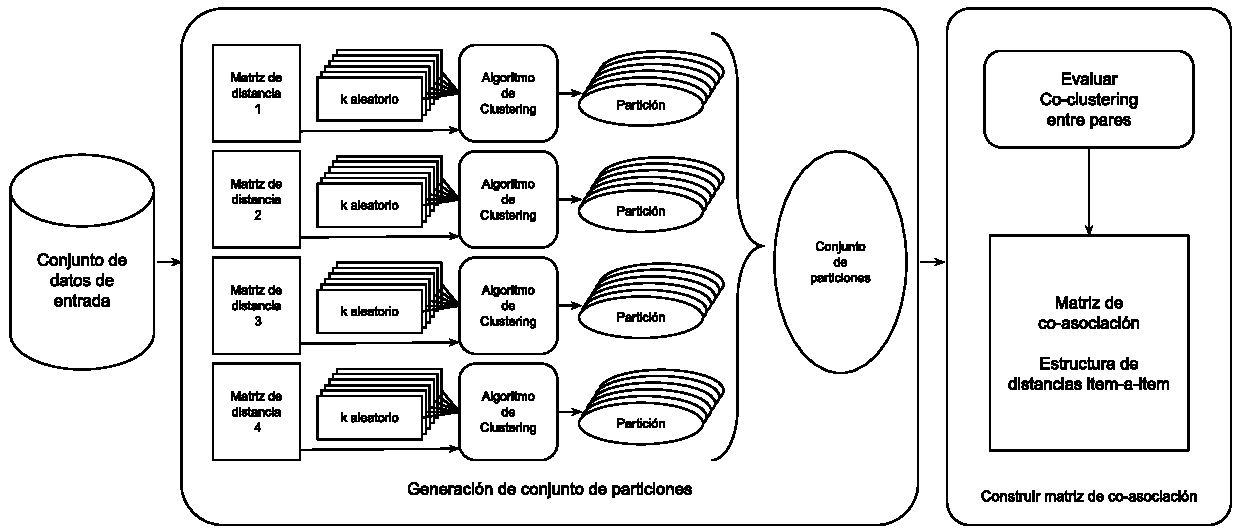
\includegraphics[width=0.9\linewidth]{8_problema_investigacion/imagenes/metodo_equal}
	\caption{Método EQuAL para la generación de matrices de co-asociación desde el conjunto de datos original.}
	\label{fig:metodoequal}
\end{figure}

 El desarrollo para este método está basado en dos pasos, como se muestra en la Figura \ref{fig:metodoequal}: \begin{enumerate*} [label=(\roman*)] \item la generación de conjunto de particiones y \item construir matriz de co-asociación. \end{enumerate*} La primera etapa muestra 4 matrices de distancias procesadas a través de un algoritmo de clustering, formando un conjunto de particiones, para luego, en la segunda etapa, ser ensambladas para formar la matriz de coasociación.

\subsubsection{Generación de conjunto de particiones}
El primer paso es la generación de un conjunto de particiones\(X = \{x_1, x_2,... , x_n\}\) . Cada una de las particiones será una matriz de similaridad \(x_i\). El procedimiento comenzará aplicando los distintos algoritmos de medidas de similaridad de texto del estado del arte al conjunto de datos de entrada. Por cada algoritmo, este procedimiento tendrá como resultado una matriz de similaridad. Cada una de las matrices de similaridad es el resultado de la combinación de todas las preguntas (individuales) de un muestreo original.

\bigskip Por cada matriz de similaridad, se aplicarán \(c\) corridas de algoritmos de clustering, cada uno con un número \(k\) de elementos seleccionados al azar, que es un parámetro de entrada del algoritmo de clustering, que representa el número de clusters que se generarán. Esta combinación de \(n\) matrices y \(c\) ejecuciones del proceso de clustering, resultará en \(n \times c\) salidas del algoritmo de clustering elegido, es decir, particiones \(P\) como resultado. Cada partición Pcontará con la asignación de cada pregunta individual con un cluster específico.

\bigskip Con el fin de resumir la estructura de cada una de las particiones generadas por los algoritmos de clustering, se combinan las particiones anteriormente obtenidas, dando lugar a un conjunto de particiones  \(\rm I\!P\). Específicamente, si en este método utilizamos 5 algoritmos de similaridad distintos aplicados a procedimientos de clustering, obtendremos, un conjunto de 5 particiones:
\[\rm I\!P = \{P^1, P^2, P^3, P^4, P^5\};\]
siendo 5 el número de particiones que conforman el conjunto que será la entrada del procedimiento de construcción de la matriz de co-asociación.

\subsubsection{Construcción de la matriz de co-asociación}
El segundo paso es construir una matriz de co-asociación a partir del conjunto de particiones \(\rm I\!P\). Para tal fin, se aplica un algoritmo de ensamble de clustering de acumulación de evidencias, que combinará cada una de estas particiones, dando como salida una matriz de co-asociación, que contiene en cada posición la proporción de veces que los elementos \(i,j\) caen juntos en el mismo grupo de la salida de clustering, a lo largo de las \(N=n \times c\) particiones.

\bigskip La matriz de co-asociación, que es una representación integrada de las relaciones subyacentes entre los datos originales, será la entrada para RS en sitios CQA. Además, tiene la característica de ser adimensional y comprende toda la variabilidad propia de los algoritmos de clustering, por lo cual, analiza la estructura de distancia item-item que es necesaria como entrada para un RS basado en contenido incorporando varios aspectos de las distancias entre elementos de texto, en lugar de usar solo una simple medida basada individualmente en aspectos de cada una de las medidas de distancia.

\bigskip El armado de matrices, la combinación de las mismas y la aplicación de estrategias estadísticas, implica un aumento significativo del volumen de datos y requiere una capacidad de cálculo intensiva. Una arquitectura Big Data que realice el procesamiento distribuido de los mismos es fundamental para este proceso. Además del volumen de datos con el cual se trabajará, se variarán distintos parámetros, tales como la medida de similaridad y valores de umbral involucrados en procesos de clustering, con el fin de obtener resultados confiables; lo cual redunda en múltiples ejecuciones de toda la solución. Debe destacarse que, en un primer momento, se implementarán experimentos basados en una infraestructura MapReduce aplicados con frameworks basados en Hadoop y cluster computing, desplegados en servidores elásticos en la nube, lo cual provee la ventaja de procesar grandes cantidades de datos en instancias dinámicamente escalables.
